\chapter{Result} \label{result}

\commento{\begin{itemize}
\item asymemtries on carbon.
\item expected rates on lead.
\item false asymmetriies result.
\item average of the asymmetries for the pmts.
\item confront with the theory.
\end{itemize}}

In this chapter we report the result obtained for the data-analysis. First we report the averaged asymmetries with and without subtracting the pmt offset. From the asymmetry results, we can compute the factor $c$ as the ratio between the final asymmetries with and without subtracting the offset. The values can be directly confronted with the ones defined in \ref{Autocalib}. We see a good agreement. All the values are in reported in ppm (part-per-million).

\begin{table}[!ht]
\centering
\subfloat[][\emph{Asimmetries, with offset not subtracted.} \label{table:NotCorrected}]{ 
\begin{tabular}{c|c|c}
\hline
 PMT   &   Average &   $\sigma$ \\
\hline
 B0    &    -19.92 &      7.7 \\
 B1    &    -19    &      7.8 \\
 B2    &    -23.42 &      8.7 \\
 A0    &     18.8  &      3.7 \\
 A1    &     16.05 &      3.4 \\
 A2    &     18.45 &      3.7 \\
 A3    &     19    &      4.2 \\
 A4    &     20.84 &      5   \\
 A5    &     22.83 &      4.9 \\
 A6    &     17.49 &      5.5 \\
 A7    &     19.24 &      6.6 \\
\hline
\end{tabular}} \qquad
\subfloat[][\emph{Asymmetries with offsets subtracted}\label{table:OffsetCorrected}]{
\begin{tabular}{lrr} 
\hline
 PMT   &   Average &   \sigma \\
\hline
 B0    &    -20.61 &      8   \\
 B1    &    -19.69 &      8   \\
 B2    &    -24.13 &      9   \\
 A0    &     24.55 &      4.2 \\
 A1    &     22.54 &      4.1 \\
 A2    &     24.37 &      4.3 \\
 A3    &     23.49 &      4.7 \\
 A4    &     24.21 &      5.4 \\
 A5    &     26.39 &      5.3 \\
 A6    &     19.82 &      5.9 \\
 A7    &     20.97 &      6.9 \\
\hline
\end{tabular}}
\qquad
\subfloat[][\emph{$c$ factor, as defined in \ref{eq:Systematic}} \label{table:Cfactor}]{
\begin{tabular}{c|c} 
\hline
 PMT   &        c \\
\hline
 B0    & 0.97 \\
 B1    & 0.96 \\
 B2    & 0.97 \\
 A0    & 0.77 \\
 A1    & 0.71 \\
 A2    & 0.76 \\
 A3    & 0.81 \\
 A4    & 0.86 \\
 A5    & 0.87 \\
 A6    & 0.88 \\
 A7    & 0.92 \\
\hline
\end{tabular}}
\caption{Averaged asymmetries over all the events. The values are corrected subtracting $\overline{A}_{I}$ and considering the effective polarization $p$ of the beam}
\end{table}

The asymmetries are shown with the errors in the following plot. The error are obtained with the formula:
\begin{align*}
\sigma = \sqrt{\frac{1}{2 N \cdot n}}
\end{align*}

To Obtain a final asymmetry for detector A and B, the asymmetries for each plot are averaged using the formula:

\begin{equation}
\overline{A_{n}} = \sum_{i = 0}^{n_{PMT}} \dfrac{ w_{i} A_{i}}{\sum_{i = 0}^{n_{PMT}} w_{i}}
\end{equation}

This is a weighted mean, and $w_{i} = \frac{1}{\sigma^{2}_{i}}$. This formula is applied to take care of the different statistical error for different pmts.

\begin{figure}[hbtp]
\centering
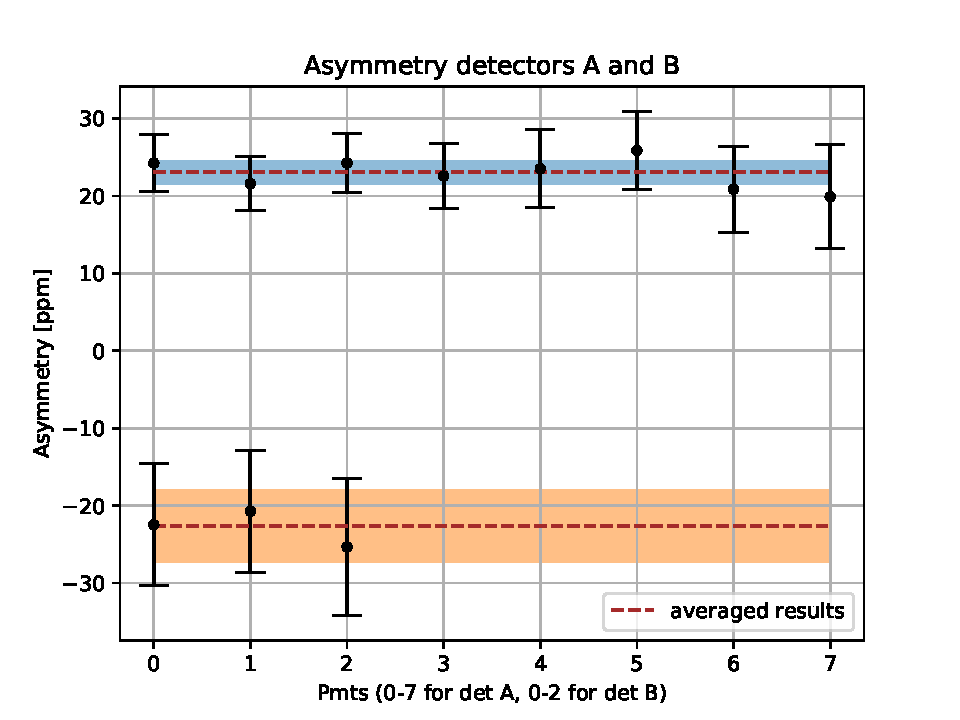
\includegraphics[width = 0.80\textwidth]{Analysis/Dataselection/FirstResult.pdf}
\caption{Plot of the asymmetries ordered by the pmt label, the result are the average event per event, corrected by the beam asymmetry current and for the polarization $p$ percentage.}
\end{figure}

The overall results for the two detectors are: 
\begin{itemize}
\item Asymmetry for detector A, $A_{A} =  23.1 \pm 1.6$ ppm.
\item Asymmetry for detector B, $A_{B} = -22.7 \pm 4.7$ ppm.
\end{itemize}

The result obtained from the linear fit of the asymmetries versus the beam parameters are reported here, together with the false asymmetry values. In this case the model is quite simple: only $X$, $Y$, $E$ are the beam parameters considered:
\begin{table}[h] \label{Tab:FitResult}
\centering
\begin{tabular}{|c|c|c|c|c|}
\hline
 PMT   & An             & Ax              & Ay                 & Ae              \\
\hline
 A0    & 23.08 $\pm$ 4.36 & 50.27 $\pm$ 27.43  & -70.44 $\pm$ 134.97  & 12.47 $\pm$ 11.57 \\
 A1    & 22.25 $\pm$ 4.18 & -7.87 $\pm$ 26.32  & -145.75 $\pm$ 129.5  & 23.52 $\pm$ 11.1  \\
 A2    & 22.21 $\pm$ 4.32 & -29.71 $\pm$ 27.2  & -78.12 $\pm$ 133.84  & 12.2 $\pm$ 11.47  \\
 A3    & 22.06 $\pm$ 4.58 & -3.13 $\pm$ 28.8   & -241.41 $\pm$ 141.72 & 2.83 $\pm$ 12.15  \\
 A4    & 23.8 $\pm$ 4.87  & 32.1 $\pm$ 30.64   & -141.52 $\pm$ 150.76 & 7.53 $\pm$ 12.92  \\
 A5    & 26.29 $\pm$ 4.91 & 13.29 $\pm$ 30.93  & 144.98 $\pm$ 152.18  & -3.39 $\pm$ 13.04 \\
 A6    & 19.09 $\pm$ 5.29 & -10.47 $\pm$ 33.29 & 88.43 $\pm$ 163.79   & 2.69 $\pm$ 14.04  \\
 A7    & 19.57 $\pm$ 5.96 & -10.63 $\pm$ 37.5  & 17.68 $\pm$ 184.52   & 19.43 $\pm$ 15.82 \\
\hline
\end{tabular}
\end{table}


\chapter{Conclusion and outlook} \label{conclusion}

\commento{\begin{itemize}
\item outlook for the future experiments with lead.
\item mention the future experiment with Parity-violatin scattering.
\end{itemize}}